\chapter{Limits \seb{$\checkmark$} }

%%% choose an epigraph to go here

\section{Encoding genealogies}

\subsection{The genealogical process}
Before we can analyse genealogies, we need a way to encode them.
The encoding will only include the information relevant to the sample genealogy, namely which lineages coalesce at which times. Information about particle positions and ``killed'' particles is ignored.

Let $\mathcal{P}_n$ be the space of partitions on $\{1,\dots,n\}$.
For convenience, we now label time in reverse, so the terminal particles are at time 0, their parents are at time 1, and so on.
Consider a randomly chosen sample of $n$ terminal particles among a total of $N$ particles, and label the sampled particles $1,\dots,n$.
The genealogical process $(G_t^{(n,N)})_{t\in\mathbb{N}_0}$ for this sample is the $\mathcal{P}_n$-valued stochastic process such that labels $i$ and $j$ are in the same block of the partition $G_t^{(n,N)}$ if and only if terminal particles $i$ and $j$ have a common ancestor at time $t$ (i.e.\ $t$ generations back).

A formulation where $G_t^{(n,N)}$ takes values in the space of equivalence relations from $[n]$ to $[n]$ is sometimes used \parencite[e.g.][]{mohle1999}; interpreting partition blocks as equivalence classes, this formulation is equivalent to ours.

The initial value of the process is the partition of singletons $G_0^{(n,N)} = \{ \{1\}, \dots, \{n\} \}$, since all of the terminal particles are in separate lineages.
The only possible non-identity transitions are those that merge some blocks of the partition, encoding the coalescence of the corresponding lineages.
The trivial partition $\{ \{1,\dots,n\} \}$ is therefore an absorbing state, corresponding to all lineages in the sample having coalesced (i.e.\ the MRCA has been reached).
The construction of the genealogical process from the resampling relationships (i.e.\ the vector of parental indices at each generation) is illustrated in Figure \ref{fig:encoding_genealogy}.

\begin{figure}
\centering
\subfloat[Resampling relationships]{
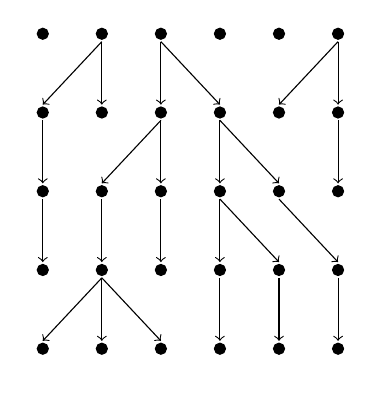
\begin{tikzpicture}
% grid of particles
\filldraw (0,0) circle (2pt);
\filldraw (0.75,0) circle (2pt);
\filldraw (1.5,0) circle (2pt);
\filldraw (2.25,0) circle (2pt);
\filldraw (3,0) circle (2pt);
\filldraw (3.75,0) circle (2pt);
\filldraw (0,1) circle (2pt);
\filldraw (0.75,1) circle (2pt);
\filldraw (1.5,1) circle (2pt);
\filldraw (2.25,1) circle (2pt);
\filldraw (3,1) circle (2pt);
\filldraw (3.75,1) circle (2pt);
\filldraw (0,2) circle (2pt);
\filldraw (0.75,2) circle (2pt);
\filldraw (1.5,2) circle (2pt);
\filldraw (2.25,2) circle (2pt);
\filldraw (3,2) circle (2pt);
\filldraw (3.75,2) circle (2pt);
\filldraw (0,3) circle (2pt);
\filldraw (0.75,3) circle (2pt);
\filldraw (1.5,3) circle (2pt);
\filldraw (2.25,3) circle (2pt);
\filldraw (3,3) circle (2pt);
\filldraw (3.75,3) circle (2pt);
\filldraw (0,4) circle (2pt);
\filldraw (0.75,4) circle (2pt);
\filldraw (1.5,4) circle (2pt);
\filldraw (2.25,4) circle (2pt);
\filldraw (3,4) circle (2pt);
\filldraw (3.75,4) circle (2pt);
% resampling arrows % generation 4 to 5
\draw[->] (0.75,0.9)--(0,0.1);
\draw[->] (0.75,0.9)--(0.75,0.1);
\draw[->] (0.75,0.9)--(1.5,0.1);
\draw[->] (2.25,0.9)--(2.25,0.1);
\draw[->] (3,0.9)--(3,0.1);
\draw[->] (3.75,0.9)--(3.75,0.1);
% resampling arrows % generation 3 to 4
\draw[->] (0,1.9)--(0,1.1);
\draw[->] (0.75,1.9)--(0.75,1.1);
\draw[->] (1.5,1.9)--(1.5,1.1);
\draw[->] (2.25,1.9)--(2.25,1.1);
\draw[->] (2.25,1.9)--(3,1.1);
\draw[->] (3,1.9)--(3.75,1.1);
% resampling arrows % generation 2 to 3
\draw[->] (0,2.9)--(0,2.1);
\draw[->] (1.5,2.9)--(0.75,2.1);
\draw[->] (1.5,2.9)--(1.5,2.1);
\draw[->] (2.25,2.9)--(2.25,2.1);
\draw[->] (2.25,2.9)--(3,2.1);
\draw[->] (3.75,2.9)--(3.75,2.1);
% resampling arrows % generation 1 to 2
\draw[->] (0.75,3.9)--(0,3.1);
\draw[->] (0.75,3.9)--(0.75,3.1);
\draw[->] (1.5,3.9)--(1.5,3.1);
\draw[->] (1.5,3.9)--(2.25,3.1);
\draw[->] (3.75,3.9)--(3,3.1);
\draw[->] (3.75,3.9)--(3.75,3.1);
% fudge bottom space
\node[anchor=north] at (0,0) {\textcolor{white}{\footnotesize{1}}};
\end{tikzpicture}
\label{fig:encoding_a}
}
\hspace{0.9cm}
\subfloat[Genealogy of terminal particles]{
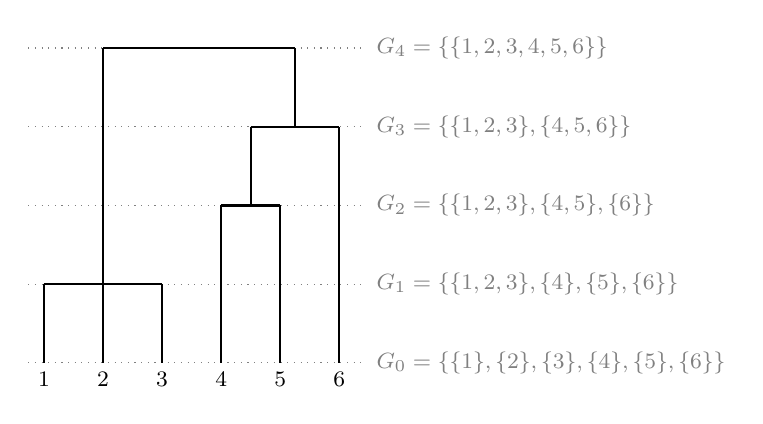
\begin{tikzpicture}
% horizontal time lines
\draw[gray,dotted] (-0.2,0)--(4.05,0);
\draw[gray,dotted] (-0.2,1)--(4.05,1);
\draw[gray,dotted] (-0.2,2)--(4.05,2);
\draw[gray,dotted] (-0.2,3)--(4.05,3);
\draw[gray,dotted] (-0.2,4)--(4.05,4);
% tree
\draw[thick] (0.75,0)--(0.75,4);
\draw[thick] (0,0)--(0,1);
\draw[thick] (1.5,0)--(1.5,1);
\draw[thick] (0,1)--(1.5,1);
\draw[thick] (2.25,0)--(2.25,2);
\draw[thick] (3,0)--(3,2);
\draw[thick] (2.25,2)--(3,2);
\draw[thick] (2.625,2)--(2.625,3);
\draw[thick] (3.75,0)--(3.75,3);
\draw[thick] (2.625,3)--(3.75,3);
\draw[thick] (3.1875,3)--(3.1875,4);
\draw[thick] (0.75,4)--(3.1875,4);
% lineage labels
\node[anchor=north] at (0,0) {\footnotesize{1}};
\node[anchor=north] at (0.75,0) {\footnotesize{2}};
\node[anchor=north] at (1.5,0) {\footnotesize{3}};
\node[anchor=north] at (2.25,0) {\footnotesize{4}};
\node[anchor=north] at (3,0) {\footnotesize{5}};
\node[anchor=north] at (3.75,0) {\footnotesize{6}};
% partition labels
\node[anchor=west] at (4.1,0) {\textcolor{gray}{\footnotesize{$G_0 = \{ \{1\}, \{2\}, \{3\}, \{4\}, \{5\}, \{6\} \}$}}};
\node[anchor=west] at (4.1,1) {\textcolor{gray}{\footnotesize{$G_1 = \{ \{1,2,3\}, \{4\}, \{5\}, \{6\} \}$}}};
\node[anchor=west] at (4.1,2) {\textcolor{gray}{\footnotesize{$G_2 = \{ \{1,2,3\}, \{4,5\}, \{6\} \}$}}};
\node[anchor=west] at (4.1,3) {\textcolor{gray}{\footnotesize{$G_3 = \{ \{1,2,3\}, \{4,5,6\} \}$}}};
\node[anchor=west] at (4.1,4) {\textcolor{gray}{\footnotesize{$G_4 = \{ \{1,2,3,4,5,6\} \}$}}};
\end{tikzpicture}
\label{fig:encoding_b}
}
\caption[Illustration of how the sample genealogy is encoded]{Illustration of how the sample genealogy is encoded. \subref{fig:encoding_a} Relationships induced by resampling in a sample of $n=6$ particles over four iterations. \subref{fig:encoding_b} The genealogy of these six particles, labelled with the value of the genealogical process $G_t$ at each time.}
\label{fig:encoding_genealogy}
\end{figure}


\subsection{Time scale}
In order to have a well-defined limit for the genealogical process as $N\to\infty$, we must scale time by a suitable function $\tau_N(\cdot)$. In the population genetics literature the time scale function is typically deterministic (Section~\ref{sec:popgenmodels}), but in our case $\tau_N$ depends on the offspring counts and is therefore random.
To define the time scale we first define the pair merger rate
\begin{equation}\label{eq:defn_cN}
c_N(t) := \frac{1}{(N)_2} \sum_{i=1}^N (\nu_t^{(i)})_2 .
\end{equation}
This is the probability, conditional on $\nu_t^{(1:N)}$, that a randomly chosen pair of lineages in generation $t$ merges exactly one generation back.
To achieve a limiting pair merger rate of 1, as in the $n$-coalescent, we rescale time by the generalised inverse
\begin{equation}\label{eq:defn_tauN}
\tau_N(t) := \inf \left\{ s \geq 1 : \sum_{r=1}^s c_N(r) \geq t \right\} .
\end{equation}
The function $\tau_N$ maps continuous to discrete time, providing the link between the discrete-time SMC dynamics and the continuous-time Kingman limit.
We will also need the following quantity, which is an upper bound on the conditional probability of a multiple merger (three or more lineages merging, or two or more simultaneous pairwise mergers):
\begin{equation}\label{eq:defn_DN}
D_N(t) := \frac{1}{N(N)_2} \sum_{i=1}^N (\nu_t^{(i)})_2
        \left\{ \nu_t^{(i)} + \frac{1}{N} \sum_{j\neq i} (\nu_t^{(j)})^2 \right\} .
\end{equation} 
This will be used to control the rate of multiple mergers, which must be dominated by the pair-merger rate as $N\to\infty$ if we are to recover a Kingman limit (in which almost surely the only non-identity transitions are pair mergers).
%Let $\nu_t^{(i)}$ be the number of offspring in generation $t$ of particle $i$ ($t \in \mathbb{N}$, $i = 1,\dots, N$).
%Let $(\mathcal{F}_t)$ be the reverse-time filtration generated by the offspring counts.
Some basic properties of $c_N$, $D_N$ and $\tau_N$ are stated in Proposition~\ref{thm:cN_properties}.
\begin{prop}\label{thm:cN_properties}
For all $t\in\mathbb{N}$, $t^\prime > s^\prime >0$,
\begin{enumerate}[label=(\alph*)]
\item \label{item:cN_property1} \hspace{5pt}
    $\begin{aligned}
    c_N(t) , D_N(t) \in [0,1]
    \end{aligned}$
\item \label{item:cN_property2} \hspace{5pt}
    $\begin{aligned}
    D_N(t) \leq c_N(t)
    \end{aligned}$
\item \label{item:cN_property3} \hspace{5pt}
    $\begin{aligned}
    c_N(t)^2 \leq c_N(t) 
    \end{aligned}$
\item \label{item:cN_property4} \hspace{5pt}
    $\begin{aligned}
    t^\prime
    \leq \sum_{r=1}^{\tau_N(t^\prime)} c_N(r) 
    \leq t^\prime +1 .
    \end{aligned}$
\item \label{item:cN_property5} \hspace{5pt}
    $\begin{aligned}
    t^\prime - s^\prime -1
    \leq \sum_{r=\tau_N(s^\prime)+1}^{\tau_N(t^\prime)} c_N(r) 
    \leq t^\prime - s^\prime +1 .
    \end{aligned}$
\item \label{item:cN_property6} \hspace{5pt}
    $\begin{aligned}
    \tau_N(t^\prime) \geq t^\prime .
    \end{aligned}$
\end{enumerate}
%\begin{align}
%& c_N(t) , D_N(t) \in [0,1] \label{eq:cN_property1}\\
%& D_N(t) \leq c_N(t) \label{eq:cN_property2}\\
%& c_N(t)^2 \leq c_N(t) \label{eq:cN_property3}\\
%& t^\prime \leq \sum_{r=1}^{\tau_N(t^\prime)} c_N(r) \leq t^\prime +1 . \label{eq:cN_property4}
%\end{align}
\end{prop}

\begin{proof}
\textbf{\ref{item:cN_property1}}  $c_N(t)$ and $D_N(t)$ are clearly non-negative. Both are maximised when one of the offspring counts is equal to $N$ and the rest are zero, in which case $c_N(t) = D_N(t) = 1$.\\
\textbf{\ref{item:cN_property2}} As outlined in \textcite[p.9]{koskela2018},
\begin{align*}
D_N(t) &:= \frac{1}{(N)_2} \sum_{i=1}^N (\nu_t^{(i)})_2 \frac{1}{N} \left\{  \nu_t^{(i)} + \frac{1}{N} \sum_{j\neq i}^N (\nu_t^{(j)})^2 \right\} \\
&\leq \frac{1}{(N)_2} \sum_{i=1}^N (\nu_t^{(i)})_2 \frac{1}{N} \left\{  \nu_t^{(i)} + \frac{1}{N} \sum_{j\neq i}^N N \nu_t^{(j)} \right\} \\
&= \frac{1}{(N)_2} \sum_{i=1}^N (\nu_t^{(i)})_2 \frac{1}{N} \left\{ \sum_{j =1}^N \nu_t^{(j)} \right\}
= \frac{1}{(N)_2} \sum_{i=1}^N (\nu_t^{(i)})_2
= c_N(t) .
\end{align*}
\textbf{\ref{item:cN_property3}} is immediate given \ref{item:cN_property1}.\\
\textbf{\ref{item:cN_property4}} follows directly from the definition of $\tau_N$ in \eqref{eq:defn_tauN}.\\
\textbf{\ref{item:cN_property5}} Writing
\begin{equation*}
\sum_{r=\tau_N(s^\prime)+1}^{\tau_N(t^\prime)} c_N(r)
= \sum_{r=1}^{\tau_N(t^\prime)} c_N(r) 
        - \sum_{r=1}^{\tau_N(s^\prime)} c_N(r) ,
\end{equation*}
the result follows by applying \ref{item:cN_property4} to both sums.\\
\textbf{\ref{item:cN_property6}} follows from \ref{item:cN_property1} and the definition of $\tau_N$ in \eqref{eq:defn_tauN}.
\end{proof}


Another useful property is the following, based on \textcite[Lemma 2]{koskela2018}. There the special case $f(r) \equiv c_N(r)$ is proved, but the authors remark that the result also holds for other choices of $f$. Here we state the result in full generality.

\begin{lemma}\label{thm:kjjslemma2}
Fix $t>0$.
Let $(\mathcal{F}_r)$ be the backwards-in-time filtration generated by the offspring counts $\nu_r^{(1:N)}$ at each generation $r$.
Let $f(r)$ be any deterministic function of $\nu_r^{(1:N)}$ such that for all $r$ there exists $B<\infty$ for which $0\leq f(r) \leq B$.
Then
\begin{equation*}
\E \left[ \sum_{r=1}^{\tau_N(t)} f(r) \right] 
= \E \left[ \sum_{r=1}^{\tau_N(t)} \E [ f(r) \mid \mathcal{F}_{r-1} ] \right] .
\end{equation*}
\end{lemma}

\begin{proof}
Define 
\begin{equation*}
M_s 
:= \sum_{r=1}^s \left\{ f(r) - \E [ f(r) \mid \mathcal{F}_{r-1} ] \right\} .
\end{equation*}
It is easy to establish that $(M_s)$ is a martingale with respect to $(\mathcal{F}_s)$, and $M_0 = 0$. 
Now fix $K\geq 1$ and note that $\tau_N(t) \wedge K$ is a bounded $\mathcal{F}_t$-stopping time.
Hence we can apply the optional stopping theorem:
\begin{align*}
\E [M_{\tau_N(t) \wedge K} ]
&= \E \left[ \sum_{r=1}^{\tau_N(t) \wedge K} \left\{ f(r) 
        - \E [ f(r) \mid \mathcal{F}_{r-1} ] \right\} \right] \\
&= \E \left[ \sum_{r=1}^{\tau_N(t) \wedge K} f(r) \right]
        - \E \left[ \sum_{r=1}^{\tau_N(t) \wedge K} 
        \E [ f(r) \mid \mathcal{F}_{r-1} ] \right]
=0 .
\end{align*}
Since this holds for all $K\geq 1$,
\begin{equation*}
\lim_{K\to\infty} \E \left[ \sum_{r=1}^{\tau_N(t) \wedge K} f(r) \right]
= \lim_{K\to\infty} \E \left[ \sum_{r=1}^{\tau_N(t) \wedge K} 
        \E [ f(r) \mid \mathcal{F}_{r-1} ] \right] .
\end{equation*}
The monotone convergence theorem allows the limit to pass inside the expectation on each side (since increasing $K$ can only increase each sum, by possibly adding some non-negative terms). Hence
\begin{align*}
\E \left[ \sum_{r=1}^{\tau_N(t)} f(r) \right]
&= \E \left[ \lim_{K\to\infty} \sum_{r=1}^{\tau_N(t) \wedge K} f(r) \right]
= \E \left[ \lim_{K\to\infty} \sum_{r=1}^{\tau_N(t) \wedge K} 
        \E [ f(r) \mid \mathcal{F}_{r-1} ] \right] \\
&= \E \left[ \sum_{r=1}^{\tau_N(t)} 
        \E [ f(r) \mid \mathcal{F}_{r-1} ] \right] ,
\end{align*}
which concludes the proof.
\end{proof}



\subsection{Transition probabilities}
%Let $\mathcal{P}_n$ be the space of partitions of $\{1,\dots,n\}$, and denote by $\Delta$ the partition of singletons $\{ \{1\},\dots, \{n\} \}$.
Recall that $\mathcal{P}_n$ denotes the space of partitions of $\{1,\dots,n\}$.
For any $\xi, \eta \in \mathcal{P}_n$ and $t\in\mathbb{N}$, let $p_{\xi\eta}(t)$ denote the conditional transition probabilities of the genealogical process given $\nu_t^{(1:N)}$. % ($t\in\mathbb{N}$, $\xi, \eta \in \mathcal{P}_n$).
The transition probability $p_{\xi\eta}(t)$ can only be non-zero when $\eta$ is obtained from $\xi$ by merging some blocks of $\xi$ (i.e.\ some lineages coalescing).
Ordering the blocks by their least element, denote by $b_i$ the number of blocks of $\xi$ that merge to form block $i$ in $\eta$, for each $i \in \{1,\dots, |\eta|\}$. Hence $b_1 + \cdots + b_{|\eta|} = |\xi|$.
Then the transition probability is given by
\begin{equation}\label{eq:defn_pxieta}
p_{\xi\eta}(t) 
:= \frac{1}{(N)_{|\xi|}} \sum_{\substack{i_1 \neq \cdots \neq i_{|\eta|} \\ =1}}^N
        (\nu_t^{(i_1)})_{b_1} \cdots (\nu_t^{(i_{|\eta|})})_{b_{|\eta|}} .
\end{equation}
We will only need to work directly with the identity transition probabilities $p_{\xi\xi}(t)$.
Upper and lower bounds on these probabilities are presented in Propositions \ref{thm:pDelta_LB} and \ref{thm:pDelta_UB}.
\begin{prop}%[Lower bound on identity transition probabilities]
\label{thm:pDelta_LB}
Let $\xi \in \mathcal{P}_n$, $N>2$. Then
\begin{equation*}
p_{\xi\xi}(t)
\geq 1 - \binom{|\xi|}{2} \frac{N^{|\xi|-2}}{(N-2)_{|\xi|-2}} \left[ c_N(t) + B_{|\xi|} D_N(t) \right]
\end{equation*}
where 
\begin{equation*}
B_{|\xi|} = K (|\xi|-1)! (|\xi|-2) \exp( 2 \sqrt{2(|\xi|-2)} )
\end{equation*}
for some $K>0$ that does not depend on $|\xi|$.
\end{prop}
%\seb{For weak convergence proof, refer to this proposition but rewrite the inequality using $\xi = \Delta$ and $\alpha_n$, to provide a local target for cross-referencing. Similarly for UB.}
\begin{proof}
%The proof follows \textcite[Proof of Lemma 3.6]{brown2021}, but keeping the terms in $N$ explicit. --- I don't need to refer to BJJK as it's part of my work; just reproduce BJJK's workings nice and verbosely here :)
We have the following expression for $p_{\xi\xi}(t)$, by subtracting all possible non-identity transitions (the omitted $k=|\xi|$ term would count identity transitions):
\begin{equation*}
p_{ \xi \xi }( t ) 
= 1 - \frac{ 1 }{ ( N )_{ | \xi | } } \sum_{ k = 1 }^{ | \xi | - 1 } 
        \sum_{ \substack{ b_1 \geq \ldots \geq b_k = 1 
        \\ b_1 + \ldots + b_k = | \xi | } }^{ | \xi | } 
        \frac{ | \xi |! }{ \prod_{ j = 1 }^{ | \xi | } ( j ! )^{ \kappa_j } \kappa_j ! } 
        \sum_{ \substack{ i_1 \neq \ldots \neq i_k = 1 \\ \text{all distinct} } }^N 
        ( \nu_t^{ ( i_1 ) } )_{ b_1 } \ldots ( \nu_t^{ ( i_k ) } )_{ b_k },
\end{equation*}
where $\kappa_i = |\{ j : b_j = i \}|$ is the multiplicity of mergers of size $i$ ($\kappa_1$ counts non-merger events, and we have the identity $\kappa_1 + 2 \kappa_2 + \cdots + | \xi | \kappa_{ | \xi | } = | \xi |$).
The combinatorial factor is the number of partitions of a sequence of length $|\xi|$  having $\kappa_j$ subsequences of length $j$ for each $j$ \parencite[Equation (11)]{fu2006}.

We separate the $k=|\xi|-1$ term (which counts single pair mergers), for which $(b_1, b_2, \dots, b_{|\xi|-1}) = (2,1,\dots,1)$ and
\begin{equation*}
\frac{ | \xi |! }{ \prod_{ j = 1 }^{ | \xi | } ( j ! )^{ \kappa_j } \kappa_j ! }
= \binom{|\xi|}{2} .
\end{equation*}
For the remaining terms we use
\begin{equation*}
\frac{ | \xi |! }{ \prod_{ j = 1 }^{ | \xi | } ( j ! )^{ \kappa_j } \kappa_j ! }
\leq |\xi|! .
\end{equation*}
Thus
\begin{align}
p_{ \xi \xi }( t ) 
&\geq 1 - \frac{ 1 }{ ( N )_{ | \xi | } } \binom{|\xi|}{2}
        \sum_{ \substack{ i_1 \neq \ldots \neq i_{|\xi|-1} = 1 \\ \text{all distinct} } }^N 
        ( \nu_t^{ ( i_1 ) } )_2 \nu_t^{(i_2)} \ldots \nu_t^{ ( i_{|\xi|-1} ) } \notag\\
    &\qquad- \frac{ 1 }{ ( N )_{ | \xi | } } \sum_{ k = 1 }^{ | \xi | - 1 } 
        \sum_{ \substack{ b_1 \geq \ldots \geq b_k = 1 
        \\ b_1 + \ldots + b_k = | \xi | } }^{ | \xi | } |\xi|!
        \sum_{ \substack{ i_1 \neq \ldots \neq i_k = 1 \\ \text{all distinct} } }^N 
        ( \nu_t^{ ( i_1 ) } )_{ b_1 } \ldots ( \nu_t^{ ( i_k ) } )_{ b_k } \label{eq:pDeltaLB_1}
\end{align}
Now, for the $k=|\xi|-1$ term we use the bound
\begin{equation*}
\sum_{ i_1 \neq \ldots \neq i_{ | \xi | - 1 } = 1 }^N 
        ( \nu_t^{ ( i_1 ) } )_2 \nu_t^{ ( i_2 ) } \ldots \nu_t^{ ( i_{ | \xi | - 1 } ) }
\leq N^{ | \xi | - 2 } \sum_{ i = 1 }^N ( \nu_t^{ ( i ) } )_2
\end{equation*}
while for the other terms we have \parencite[similarly to][Lemma 1 Case 3]{koskela2018}
\begin{align*}
\sum_{ \substack{ i_1 \neq \ldots \neq i_k = 1 \\ \text{all distinct} } }^N &( \nu_t^{ ( i_1 ) } )_{ b_1 } \ldots ( \nu_t^{ ( i_k ) } )_{ b_k } \leq \sum_{ i = 1 }^N ( \nu_t^{ ( i ) } )_2 \Bigg( N^{ | \xi | - 2 } - \sum_{ \substack{ j_1 \neq \ldots \neq j_{ | \xi | - 2 } = 1 \\ \text{all distinct and } \neq i } }^N \nu_t^{ ( j_1 ) } \ldots \nu_t^{ ( j_{ | \xi | - 2 } ) } \Bigg) \\
&\leq \sum_{ i = 1 }^N ( \nu_t^{ ( i ) } )_2 \Bigg\{ N^{ | \xi | - 2 } - ( N - \nu_t^{ ( i ) } )^{ | \xi | - 2 } + \binom{ | \xi | - 2 }{ 2 } \sum_{ j \neq i } ( \nu_t^{ ( j ) } )^2 \Bigg( \sum_{ k \neq i } \nu_t^{ ( k ) } \Bigg)^{ | \xi | - 4 } \Bigg\} \\
&\leq \sum_{ i = 1 }^N ( \nu_t^{ ( i ) } )_2 \Bigg\{ ( | \xi | - 2 ) \nu_t^{ ( i ) } N^{ | \xi | - 3 } + \binom{ | \xi | - 2 }{ 2 } \sum_{ j \neq i } ( \nu_t^{ ( j ) } )^2 N^{ | \xi | - 4 } \Bigg\},
\end{align*}
where the last step uses $(N - x)^b \geq N^b - b x N^{ b - 1 }$ for $x \leq N$, $b \geq 0$.
Hence
\begin{align*}
p_{ \xi \xi }( t ) 
&\geq 1 - \frac{ 1 }{ ( N )_{ | \xi | } } \binom{|\xi|}{2}
        N^{ | \xi | - 2 } \sum_{ i = 1 }^N ( \nu_t^{ ( i ) } )_2 \\
    &\qquad- \frac{ N^{|\xi|-3} }{ ( N )_{ | \xi | } } |\xi|!
        \sum_{ k = 1 }^{ | \xi | - 1 } 
        \sum_{ \substack{ b_1 \geq \ldots \geq b_k = 1 
        \\ b_1 + \ldots + b_k = | \xi | } }^{ | \xi | } 
        \sum_{ i = 1 }^N ( \nu_t^{ ( i ) } )_2 
        \Bigg\{ ( | \xi | - 2 ) \nu_t^{ ( i ) } + \binom{ | \xi | - 2 }{ 2 } \frac{1}{N} 
        \sum_{ j \neq i } ( \nu_t^{ ( j ) } )^2 \Bigg\} .
\end{align*}
The summands in the last line are independent of $k, b_1, \dots, b_k$, and the number of terms in the sums over $k$ and $b_1, \dots, b_k$ is bounded by $\gamma_{|\xi|-2} (|\xi|-2)$, where $\gamma_n$ is the number of integer partitions of $n$.
By \textcite[Section 2]{hardy1918}, $\gamma_n < K e^{ 2 \sqrt{ 2 n } } / n$ for a constant $K > 0$ independent of $n$.
Thus, for $|\xi| > 2$,
\begin{align*}
p_{ \xi \xi }( t ) 
&\geq 1 - \frac{ N^{ | \xi | - 2 } }{ ( N-2 )_{ | \xi | -2} } \binom{|\xi|}{2}
        c_N(t) \\
    &\qquad- \frac{ N^{|\xi|-2} }{ ( N-2 )_{ | \xi | -2} }
        K \exp( 2 \sqrt{2(|\xi|-2)} ) |\xi|!
        \frac{1}{N(N)_2} \\
    &\hspace{4cm} \sum_{ i = 1 }^N ( \nu_t^{ ( i ) } )_2
        \Bigg\{ ( | \xi | - 2 ) \nu_t^{ ( i ) } + \binom{ | \xi | - 2 }{ 2 } \frac{1}{N} 
        \sum_{ j \neq i } ( \nu_t^{ ( j ) } )^2 \Bigg\} \\
&\geq 1 - \frac{ N^{ | \xi | - 2 } }{ ( N-2 )_{ | \xi | -2} } \binom{|\xi|}{2}
        c_N(t) \\
    &\qquad- \frac{ N^{|\xi|-2} }{ ( N-2 )_{ | \xi | -2} }
        K \exp( 2 \sqrt{2(|\xi|-2)} ) |\xi|! \binom{ |\xi|-1}{2} D_N(t) \\
&\geq 1 - \frac{ N^{ | \xi | - 2 } }{ ( N-2 )_{ | \xi | -2} } \binom{|\xi|}{2}
        \left[ c_N(t) + B_{|\xi|} D_N(t) \right]
\end{align*}
where
\begin{align*}
B_{|\xi|} 
&= \binom{|\xi|}{2}^{-1} K \exp( 2 \sqrt{2(|\xi|-2)} ) |\xi|! \binom{ |\xi|-1}{2} \\
&= K (|\xi|-1)! (|\xi|-2) \exp( 2 \sqrt{2(|\xi|-2)} ) .
\end{align*}
%When $|\xi| \leq 2$, there are no terms with $k\leq |\xi|-2$, and the result is immediate.
When $|\xi| = 2$, \eqref{eq:pDeltaLB_1} becomes 
\begin{equation*}
p_{ \xi \xi }( t )
\geq 1 - c_N(t)
\end{equation*}
and when $|\xi| = 1$, 
\eqref{eq:pDeltaLB_1} becomes 
\begin{equation*}
p_{ \xi \xi }( t )
\geq 1 ;
\end{equation*}
in both cases the result is immediate.
\end{proof}


\begin{prop}%[Upper bound on identity transition probabilities]
\label{thm:pDelta_UB}
Let $\xi \in \mathcal{P}_n$. Then, for $N$ sufficiently large,
\begin{equation*}
p_{\xi\xi}(t)
\leq 1 - \binom{|\xi|}{2} \{ 1 + O(N^{-1}) \} 
        \left[ c_N(t) - B_{|\xi|}^\prime D_N(t) \right]
\end{equation*}
where $B_{|\xi|}^\prime = \binom{|\xi|-1}{2}$.
\end{prop}

A proof is given in \textcite[Lemma 1 Case 1]{koskela2018}.\seb{refer to the erratum once available, which is more explicit about this proof.}





\section{An existing limit theorem}
Under the assumption \ref{standing_assumption} stated below, it is sufficient for our purposes to consider only offspring counts $\nu_t^{(1:N)} = (\nu_t^{(1)},\dots,\nu_t^{(N)})$, where $\nu_t^{(i)} = |\{ j: a_t^{(j)} =i \}|$, rather than the parental indices $a_t^{(1:N)}$ which are generally more informative.

\begin{enumerate}[label=(A\arabic*)]
\item\label{standing_assumption} The conditional distribution of parental indices $a_t^{(1:N)}$ given offspring counts $\nu_t^{(1:N)}$ is uniform over all assignments such that $ |\{ j: a_t^{(j)} =i \}|= \nu_t^{(i)} $ for all $i$.
%valid assignments.
\end{enumerate}
As we saw in Section~\ref{sec:coaltheory}, the $n$-coalescent is \emph{exchangeable}, so for instance the pair of lineages merging at each event is chosen uniformly. 
\ref{standing_assumption} is a weaker condition than exchangeability of the particles within a generation which is sufficient to admit an exchangeable process in the limit.
Exchangeability of the particles would imply neutrality, an unreasonable assumption in the setting of SMC. 
In contrast, \ref{standing_assumption} can easily be enforced upon any SMC algorithm by applying a random permutation to the offspring indices immediately after resampling.
%, without qualitatively affecting the dynamics.


\textcite{koskela2018} proved the following theorem which gives sufficient conditions under which sampled genealogies of (non-neutral) interacting particle systems converge to the $n$-coalescent as $N\to\infty$.
Naturally, such a result can only be expected to hold for genealogies of finite samples ($n<<N$), and not for the entire genealogy of the $N$ particles. 
For instance the genealogies arising in SMC algorithms are not restricted to single pair mergers only, although within a sparse sample we may, under mild conditions, see only single pair mergers. 
That is to say, there is not an extension of this result whereby the whole-population genealogy converges to the Kingman coalescent as $N\to\infty$, unless very restrictive conditions are imposed.

\begin{theorem}[\cite{koskela2018}]\label{thm:kjjs_mainthm}
Fix $n \leq N$ as the observed number of particles from the output of an interacting particle system with $N$ particles which satisfies \ref{standing_assumption}.
Suppose that for any $0 \leq s < t < \infty$, we have
\begin{gather}\label{eq:kjjs_big_merger_bound}
\lim_{ N \rightarrow \infty } \E\Bigg[ \sum_{ r = \tau_N( s ) + 1 }^{ \tau_N( t ) } D_N( r ) \Bigg] = 0, \\
%\end{equation}
%\begin{equation}
\label{eq:kjjs_binary_bound}
\lim_{ N \rightarrow \infty } \E[ c_N( t ) ] = 0, \\
%\end{equation}
%\begin{equation}
\label{eq:kjjs_binary_bound_2}
\lim_{ N \rightarrow \infty } \E\Bigg[ \sum_{ r = \tau_N( s ) + 1 }^{ \tau_N( t ) } c_N( r )^2 \Bigg] = 0, \\
%\end{equation}
%and
%\begin{equation}
\label{eq:kjjs_tau_bound}
\text{and}\qquad\qquad\E[ \tau_N( t ) - \tau_N( s ) ] \leq C_{ t, s } N,\qquad\qquad\phantom{\text{and}}
\end{gather}
for some constant $C_{ t, s } > 0$ that is independent of $N$.
Then $( G_{ \tau_N( t ) }^{ ( n, N ) } )_{ t \geq 0 }$ converges to the Kingman $n$-coalescent in the sense of finite-dimensional distributions as $N \rightarrow \infty$. 
\end{theorem}

To ensure samples of size $n$ have Kingman genealogies in the limit, with pair mergers only, we require that multiple mergers (that is, where more than two lineages merge into one, or where two or more mergers happen simultaneously) occur on a slower time scale than pair mergers. 
This is the role of condition \eqref{eq:kjjs_big_merger_bound}.

Conditions \eqref{eq:kjjs_binary_bound} and \eqref{eq:kjjs_binary_bound_2} ensure that the limiting process is continuous and has the required unit pair merger rate.
%, and will not be violated by any reasonable SMC algorithm. 
For \eqref{eq:kjjs_binary_bound} to fail to hold, the expected number of mergers at some generation would have to be $O(N^2)$. This can only happen if the resampling scheme is very bad (e.g.\ star resampling) or the weights are particularly badly-behaved. The latter is ruled out in the corollaries of Chapter~\ref{ch:appl} by imposing bounds on the potential functions; this is discussed further in Section~??\seb{add reference once that part is written}.

Condition \eqref{eq:kjjs_tau_bound} specifies that the time scale must be $O(N)$. As we saw in Section~\ref{sec:popgenmodels}, this is the correct time scale for the Wright-Fisher model, but for instance the Moran model has time scale $O(N^2)$ and hence violates this condition. 
Since we know that the neutral Moran model also has Kingman genealogies in the limit, condition \eqref{eq:kjjs_tau_bound} clearly is not necessary. 
The simplified statement in Theorem~\ref{thm:FDDconv} does not impose any such condition on the time scale.

The proof of \textcite{koskela2018} does not explicitly use \eqref{eq:kjjs_binary_bound} but rather the similar condition
\begin{equation}\label{eq:kjjs_binary_bound_corrected}
\lim_{ N \rightarrow \infty } \E[ c_N( \tau_N(t) ) ] = 0 .
\end{equation}
However, as we will see in the next section (Lemmata \ref{thm:DNimpliescN} and \ref{thm:DNimpliescN_2}), both \eqref{eq:kjjs_binary_bound} and \eqref{eq:kjjs_binary_bound_corrected} are implied by \eqref{eq:kjjs_big_merger_bound}, so the theorem is correct. 
Such redundancies in the statement of Theorem~\ref{thm:kjjs_mainthm} are removed in Theorem~\ref{thm:FDDconv}.

%%%%

The proof of Theorem~\ref{thm:kjjs_mainthm} \parencite[i.e.][Theorem 1]{koskela2018} proceeds in three parts.
The first is a vanishing upper bound on finite-dimensional distributions of the genealogical process when the path of the process involves any multiple mergers.
%, either multiple simultaneous mergers or any merger involving more than two particles.
The second is showing that, when the path of the genealogy consists of only single pair mergers, the finite-dimensional distributions of the $n$-coalescent upper bound those of the genealogical process in the limit $N\to\infty$.
The final piece is a similar lower bound, which together with the upper bound establishes convergence of the finite-dimensional distributions.




\section{A new limit theorem}
We now present a related theorem, having the same conclusion but with conditions that are more tractable and remove some redundancies in the statement of Theorem~\ref{thm:kjjs_mainthm}. 
While we do not prove that this is a strict generalisation, there are certainly systems which satisfy the conditions of Theorem~\ref{thm:FDDconv} but not of Theorem~\ref{thm:kjjs_mainthm}.

\begin{theorem}\label{thm:FDDconv}
Let $\nu_t^{(1:N)}$ denote the offspring numbers in an interacting particle system satisfying \ref{standing_assumption} such that, for any $N$ sufficiently large, $\Prob[ \tau_N(t) = \infty ] =0$ for all finite $t$. Suppose that there exists a deterministic sequence $(b_N)_{N\geq1}$ such that ${\lim}_{N\to\infty} b_N =0$ and
\begin{equation}\label{eq:mainthmcond}
\frac{1}{(N)_3} \sum_{i = 1}^N \Et[ (\nu_t^{(i)})_3 ]  \leq b_N \frac{1}{(N)_2} \sum_{i = 1}^N \Et[ (\nu_t^{(i)})_2 ]
\end{equation}
for all $N$, uniformly in $t \geq 1$.
Fix $n\leq N$ and consider a randomly chosen sample of $n$ terminal particles.
Then the resulting rescaled genealogical process $(G_{\tau_N(t)}^{(n,N)})_{t\geq0}$ converges in the sense of finite-dimensional distributions to Kingman's $n$-coalescent as $N \to \infty$.
\end{theorem}

On the RHS of \eqref{eq:mainthmcond} is the filtered expectation of $c_N(t)$, i.e.\ the expected pair merger rate, and the LHS is the corresponding rate of triple mergers. Intuitively, \eqref{eq:mainthmcond} says that pair mergers dominate triple mergers, the expected rate of which vanishes as $N\to\infty$. As we will see, this implies that pair mergers also dominate all other larger mergers, such as simultaneous pair mergers.

Our result improves on Theorem~\ref{thm:kjjs_mainthm} by eliminating the restrictive condition \eqref{eq:kjjs_tau_bound}, which 
%is shown in Lemma~\ref{lem:removeass4}\seb{?!} to be 
we know is unnecessary. This allows our result to apply to some models not previously included; for example the neutral Moran model. %violates \eqref{eq:kjjs_tau_bound} but is included in Theorem~\ref{thm:FDDconv}. 
Although we do not prove that Theorem~\ref{thm:FDDconv} is a true generalisation of Theorem~\ref{thm:kjjs_mainthm}, \textcite[Theorem 5.4]{mohle2003} showed that in neutral models the straightforward analogue of \eqref{eq:mainthmcond} is both necessary and sufficient, suggesting that in general this condition is not significantly stronger than \eqref{eq:kjjs_big_merger_bound}--\eqref{eq:kjjs_binary_bound_2} combined.

Our conditions are also significantly easier to verify than those of Theorem~\ref{thm:kjjs_mainthm}. Not only are four conditions replaced with one, but the condition \eqref{eq:mainthmcond} only involves marginal moments of the offspring counts, whereas \eqref{eq:kjjs_big_merger_bound} and \eqref{eq:kjjs_binary_bound_2} involve mixed moments. 
As we will see in Chapter~4, once we move beyond conditionally independent resampling schemes such as multinomial resampling, the joint distributions of offspring counts become complex and it may only be feasible to calculate their moments marginally. 
As such, we are able to verify the conditions of Theorem~\ref{thm:FDDconv} in several cases, including for resampling schemes that induce strong correlations between offspring counts, whereas \textcite{koskela2018} apply their theorem only to multinomial resampling.

Our condition on the time scale, $\Prob[ \tau_N(t) = \infty ] =0$, is not very restrictive. Essentially, it rules out systems in which coalescences occur at only finitely many generations. 
This condition is not actually necessary for Theorem~\ref{thm:FDDconv} to hold, as such, but if it is violated then the limiting object is an $n$-coalescent under an infinite time-scaling, that is $n$ lineages never coalescing.
This would constitute a qualitatively different result and one that is of little interest for SMC, so we follow \textcite{mohle1998} in excluding it.


\subsection{Proof of theorem}
%The series of Lemmata \ref{lem:removeass3}--\ref{lem:removeass2} below show that the assumptions \eqref{eq:oldass1}--\eqref{eq:oldass3} follow from \eqref{eq:mainthmcond}. Lemma \ref{lem:removeass4} allows us to remove condition \eqref{eq:oldass4} by improving upon some arguments from the proof of \textcite[Theorem 1]{koskela2018}; this argument is presented in detail in Section~\ref{sec:proof}.

First we prove that \eqref{eq:kjjs_binary_bound_corrected} and the assumptions \eqref{eq:kjjs_big_merger_bound}--\eqref{eq:kjjs_binary_bound_2} of Theorem~\ref{thm:kjjs_mainthm} all follow from \eqref{eq:mainthmcond}.
Figure~\ref{fig:FDD_proof_dependencies} illustrates how the following Lemmata \ref{lem:removeass3}--\ref{lem:removeass2} fit together. 
The argument differs slightly from that presented in \textcite{brown2021} in that we will here show $\eqref{eq:mainthmcond} \Rightarrow \eqref{eq:kjjs_big_merger_bound} \Rightarrow \eqref{eq:kjjs_binary_bound}$ rather than $\eqref{eq:mainthmcond} \Rightarrow \eqref{eq:kjjs_big_merger_bound}$ and $\eqref{eq:mainthmcond} \Rightarrow \eqref{eq:kjjs_binary_bound}$.
This highlights the redundancy in Theorem~\ref{thm:kjjs_mainthm}, where condition \eqref{eq:kjjs_big_merger_bound} directly implies two of the other stated conditions.

The second step in the proof is to show that condition \eqref{eq:kjjs_tau_bound} is not necessary. In particular, the parts of the proof of \textcite{koskela2018} which relied on \eqref{eq:kjjs_tau_bound} are rewritten using Proposition~\ref{thm:pDelta_LB} instead. 
Proposition~\ref{thm:pDelta_LB} is a lower bound on the probability of an identity transition, which holds in general without the need for further conditions, so we really are removing condition \eqref{eq:kjjs_tau_bound} rather than substituting it for a different condition.


\begin{figure}[ht]
\centering
\begin{tikzpicture}[
mynode/.style={rectangle, rounded corners, fill=gray!20, minimum size=5mm},
]
% nodes
\node[mynode] at (0,0) {\eqref{eq:mainthmcond}};
\node[mynode] at (4,0) {\eqref{eq:kjjs_big_merger_bound}};
\node[mynode] at (4,2) {\eqref{eq:kjjs_binary_bound_2}};
\node[mynode] at (8,0) {\eqref{eq:kjjs_binary_bound_corrected}};
\node[mynode] at (4,-2) {\eqref{eq:kjjs_binary_bound}};
% arrows
\draw[->, thick] (0.6,0)-- node[anchor=south] 
        {\footnotesize{Lemma~\ref{lem:removeass2}}} (3.5,0);
\draw[->, thick] (4,0.3)-- node[anchor=west] 
        {\footnotesize{Lemma~\ref{lem:removeass3}}} (4,1.7);
\draw[->, thick] (4.5,0)-- node[anchor=south] 
        {\footnotesize{Lemma~\ref{thm:DNimpliescN_2}}} (7.5,0);
\draw[->, thick] (4,-0.3)-- node[anchor=west] 
        {\footnotesize{Lemma~\ref{thm:DNimpliescN}}} (4,-1.7);
\draw[->, thick, gray] (0.6,0)-- node[sloped, anchor=center, text width=2cm] 
        {\textcolor{gray}{\footnotesize{Brown~et~al.~2021 Lemma 3.4}}} (3.5,-2);
\end{tikzpicture}
\caption[Dependencies between conditions of Theorems \ref{thm:kjjs_mainthm} and \ref{thm:FDDconv}]{Dependencies between conditions of Theorems \ref{thm:kjjs_mainthm} and \ref{thm:FDDconv}. Arrows represent logical implication; labels on arrows indicate the lemma in which the implication is stated.
In \textcite[Lemma 3.4]{brown2021} the direct implication \eqref{eq:mainthmcond} $\Rightarrow$ \eqref{eq:kjjs_binary_bound} was proved, but here we will instead show that \eqref{eq:kjjs_big_merger_bound} $\Rightarrow$ \eqref{eq:kjjs_binary_bound}.
}
%The main condition of Theorem~\ref{thm:FDDconv}, \eqref{eq:mainthmcond}, implies the conditions \eqref{eq:kjjs_big_merger_bound}--\eqref{eq:kjjs_binary_bound} of Theorem~\ref{thm:kjjs_mainthm}.}
\label{fig:FDD_proof_dependencies}
\end{figure}


\begin{lemma} \label{lem:removeass3}
%$\eqref{eq:kjjs_big_merger_bound} \Rightarrow \eqref{eq:kjjs_binary_bound_2}$.\\
If for all $0 \leq s < t < \infty$
\begin{equation*}
\lim_{ N \rightarrow \infty } \E\Bigg[ \sum_{ r = \tau_N( s ) + 1 }^{ \tau_N( t ) } D_N( r ) \Bigg] = 0
\end{equation*}
then for all $0 \leq s < t < \infty$
\begin{equation*}
\lim_{ N \rightarrow \infty } \E\Bigg[ \sum_{ r = \tau_N( s ) + 1 }^{ \tau_N( t ) } c_N( r )^2 \Bigg] = 0 .
\end{equation*}
\end{lemma}

\begin{proof}
%It is sufficient to show that $c_N( t )^2 \leq D_N( t ) N/(N-1)$.
We have
\begin{align*}
c_N( t )^2 &= \frac{ 1 }{ N ( N - 1 ) ( N )_2 } \sum_{ i = 1 }^N ( \nu_t^{(i)})_2 \Bigg\{ \nu_t^{(i)} ( \nu_t^{(i)} - 1 ) + \sum_{\substack{j=1\\ j \neq i }}^N ( \nu_t^{(j)} )_2 \Bigg\} \\
&= \frac{ 1 }{ N ( N )_2 } \sum_{ i = 1 }^N ( \nu_t^{(i)} )_2 \Bigg\{ \frac{ \nu_t^{(i)} ( \nu_t^{(i)} - 1 ) }{ N - 1 } + \frac{ 1 }{ N - 1 } \sum_{\substack{j=1\\ j \neq i }}^N ( \nu_t^{(j)} )_2 \Bigg\} \\
&\leq \frac{ 1 }{ N ( N )_2 } \sum_{ i = 1 }^N ( \nu_t^{(i)})_2 \Bigg\{ \nu_t^{(i)} + \frac{ 1 }{ N - 1 } \sum_{\substack{j=1\\ j \neq i }}^N ( \nu_t^{(j)} )_2 \Bigg\} \\
&\leq \frac{ 1 }{ N ( N )_2 } \sum_{ i = 1 }^N ( \nu_t^{(i)})_2 \Bigg\{ \nu_t^{(i)} + \frac{ N / ( N - 1 ) }{ N } \sum_{\substack{j=1\\ j \neq i }}^N ( \nu_t^{(j)} )^2 \Bigg\} \\
&\leq \frac{ N / ( N - 1 ) }{ N ( N )_2 } \sum_{ i = 1 }^N ( \nu_t^{(i)})_2 \Bigg\{ \nu_t^{(i)} + \frac{ 1 }{ N } \sum_{\substack{j=1\\ j \neq i }}^N ( \nu_t^{(j)} )^2 \Bigg\} = \frac{ N }{ N - 1 } D_N( t )
\end{align*}
which is sufficient for the result.
\end{proof}


\begin{lemma} \label{thm:DNimpliescN}
%\eqref{eq:kjjs_big_merger_bound} $\Rightarrow$ \eqref{eq:kjjs_binary_bound}.\\
If for all $0 \leq s < t < \infty$
\begin{equation*}
\lim_{ N \rightarrow \infty } \E\Bigg[ \sum_{ r = \tau_N( s ) + 1 }^{ \tau_N( t ) } D_N( r ) \Bigg] = 0
\end{equation*}
then for all $ t \in \mathbb{N} $
\begin{equation*}
\lim_{ N \rightarrow \infty } \E[ c_N( t ) ] = 0 .
\end{equation*}
\end{lemma}

\begin{proof}
Fix $\epsilon>0$, and assume $N>2/\epsilon$.
Following \textcite{mohle2003}, define the events
\begin{equation}\label{eq:define_Ai_events}
A_i(t) := \{ \nu_t^{(i)} \leq N\epsilon \} .
\end{equation}
Then
\begin{align*}
c_N(t)
&= \frac{1}{(N)_2} \sum_{i=1}^N (\nu_t^{(i)})_2 [\1{A_i(t)} + \1{A_i(t)^c}] \\
&\leq \frac{N\epsilon}{(N)_2} \sum_{i=1}^N \nu_t^{(i)}
        + \sum_{i=1}^N \1{A_i(t)^c} \\
&= \frac{N\epsilon}{N-1} + \sum_{i=1}^N \1{A_i(t)^c} .
\end{align*}
Taking expectations and applying the generalised Markov inequality,
\begin{align*}
\E[c_N(t)]
&\leq \epsilon\ON + \sum_{i=1}^N \Prob[ \nu_t^{(i)} > N\epsilon ] \\
&\leq \epsilon\ON 
        + \sum_{i=1}^N \frac{\E[ (\nu_t^{(i)})_3 ]}{(N\epsilon)_3} \\
&\leq \epsilon\ON + \frac{N(N)_2}{(N\epsilon)_3} \E[ D_N(t) ] \\
&= \epsilon\ON + \epsilon^{-3}\ON \E[ D_N(t) ] \\
&\leq \epsilon\ON + \epsilon^{-3}\ON 
        \E\left[ \sum_{r=1}^t D_N(r) \right] \\
&\leq \epsilon\ON + \epsilon^{-3}\ON
        \E\left[ \sum_{r=\tau_N(0)+1}^{\tau_N(t)} D_N(r) \right] .
\end{align*}
Taking limits, 
\begin{equation}
\lim_{N\to\infty} \E[c_N(t)] \leq \epsilon .
\end{equation}
Since $\epsilon$ was arbitrary this concludes the proof.
\end{proof}


\begin{lemma} \label{thm:DNimpliescN_2}
%\eqref{eq:kjjs_big_merger_bound} $\Rightarrow$ \eqref{eq:kjjs_binary_bound_corrected}.\\
If for all $0 \leq s < t < \infty$
\begin{equation*}
\lim_{ N \rightarrow \infty } \E\Bigg[ \sum_{ r = \tau_N( s ) + 1 }^{ \tau_N( t ) } D_N( r ) \Bigg] = 0
\end{equation*}
then for all $ 0 < t < \infty $
\begin{equation*}
\lim_{ N \rightarrow \infty } \E[ c_N( \tau_N(t) ) ] = 0 .
\end{equation*}
\end{lemma}

\begin{proof}
Analogously to the proof of Lemma~\ref{thm:DNimpliescN}, we find
\begin{align*}
\E[c_N(\tau_N(t))]
&\leq \epsilon\ON + \sum_{i=1}^N \Prob[ \nu_{\tau_N(t)}^{(i)} > N\epsilon ] \\
&\leq \epsilon\ON + \epsilon^{-3}\ON \E\left[ D_N(\tau_N(t)) \right] \\
&\leq \epsilon\ON + \epsilon^{-3}\ON
        \E\left[ \sum_{r=\tau_N(0)+1}^{\tau_N(t)} D_N(r) \right] \\
&\underset{N\to\infty}{\longrightarrow} \epsilon
\end{align*}
which concludes the proof.
\end{proof}


%\begin{lemma} \label{lem:removeass1}
%$\eqref{eq:mainthmcond} \Rightarrow \eqref{eq:kjjs_binary_bound}$.
%\end{lemma}
%\seb{This lemma is obsolete. In Figure \ref{fig:FDD_proof_dependencies} I'll just refer to the proof in BJJK.}
%\begin{proof}
%Following the proof of \textcite[Lemma 5.5]{mohle2003}, we fix $\varepsilon > 0$ and define the event $A_i = \{ \nu_t^{(i)} \leq N \varepsilon \}$.
%Now
%\begin{align}
%\Et[ c_N( t ) ] 
%&= \frac{ 1 }{ ( N )_2 } \sum_{ i = 1 }^N \Et[ ( \nu_t^{(i)} )_2] 
%        = \frac{ 1 }{ ( N )_2 } \sum_{ i = 1 }^N \Big\{ \Et[ ( \nu_t^{(i)} )_2 \1{ A_i } ] 
%        + \Et[ ( \nu_t^{(i)} )_2 \1{ A_i^c } ] \Big\} \notag \\
%&\leq \frac{ \varepsilon }{ N - 1 } \sum_{ i = 1 }^N \Et[ \nu_t^{(i)} \1{ A_i }] 
%        + \sum_{ i = 1 }^N \Et[\1{ A_i^c }] \notag \\
%&\leq ( 1 + O( N^{ -1 } ) ) \varepsilon + \sum_{ i = 1 }^N 
%        \Prob[ \nu_t^{(i)} > N \varepsilon \mid \mathcal{F}_{t-1}]. \label{cond_cN}
%\end{align}
%For $N \geq 3 / \varepsilon$, Markov's inequality yields
%\begin{align}
%\sum_{ i = 1 }^N \Prob[ \nu_t^{(i)} > N \varepsilon \mid \mathcal{F}_{t-1} ] 
%&\leq \frac{ 1 }{ ( N \varepsilon )_3 } \sum_{ i = 1 }^N 
%        \Et[ ( \nu_t^{(i)} )_3] 
%        = \frac{ ( 1 + O( N^{ -1 } ) ) }{ \varepsilon^3 ( N )_3 } 
%        \sum_{ i = 1 }^N \Et[ ( \nu_t^{(i)} )_3] \notag \\
%&\leq ( 1 + O( N^{ -1 } ) ) \frac{ b_N }{ \varepsilon^3 } \Et[ c_N( t )] . \label{markovs_ineq}
%\end{align}
%Substituting \eqref{markovs_ineq} into \eqref{cond_cN} and using $c_N( t ) \leq 1$ results in
%\begin{equation*}
%\Et[ c_N( t )]
%\leq ( 1 + O( N^{ -1 } ) ) 
%        \Bigg( \varepsilon + \frac{ b_N }{ \varepsilon^3 } \Bigg) \underset{N\to\infty}{\longrightarrow} \varepsilon
%\end{equation*}
%since $b_N \rightarrow 0$. 
%As $\varepsilon > 0$ was arbitrary, we have
%\begin{equation*}
%\E[ c_N( t ) ] 
%= \E\left[ \Et[ c_N( t ) ] \right] 
%\rightarrow 0
%\end{equation*}
%as $N \rightarrow \infty$.
%\end{proof}



\begin{lemma} \label{lem:removeass2}
%$\eqref{eq:mainthmcond} \Rightarrow \eqref{eq:kjjs_big_merger_bound}$.\\
If there exists a deterministic sequence $(b_N)_{N\geq1}$ such that ${\lim}_{N\to\infty} b_N =0$ and
\begin{equation*}
\frac{1}{(N)_3} \sum_{i = 1}^N \Et[ (\nu_t^{(i)})_3 ]  \leq b_N \frac{1}{(N)_2} \sum_{i = 1}^N \Et[ (\nu_t^{(i)})_2 ]
\end{equation*}
for all $N$, uniformly in $t \in \mathbb{N}$,
then for all $0 \leq s < t < \infty$
\begin{equation*}
\lim_{ N \rightarrow \infty } \E\Bigg[ \sum_{ r = \tau_N( s ) + 1 }^{ \tau_N( t ) } D_N( r ) \Bigg] = 0 .
\end{equation*}
\end{lemma}

\begin{proof}
We decompose $D_N(t)$ as the sum of two terms and consider their filtered expectations. The first is
\begin{align}
\frac{ 1 }{ N ( N )_2 } \sum_{ i = 1 }^N \Et[ ( \nu_t^{(i)} )_2 \nu_t^{(i)} ] 
&= \frac{ 1 }{ N ( N )_2 } \sum_{ i = 1 }^N 
        \Et[ 2 ( \nu_t^{(i)} )_2 + ( \nu_t^{(i)} )_3] \notag\\
&\leq \frac{ 2 }{ N } \Et[ c_N( t )] + \frac{ 1 }{ ( N )_3 } \sum_{ i = 1 }^N 
        \Et[ ( \nu_t^{(i)} )_3 ] \notag\\
&\leq \Bigg(\frac{ 2 }{ N } + b_N \Bigg) \Et[ c_N( t ) ]. \label{DN_part_1}
\end{align}
The second is
\begin{align}
\frac{ 1 }{ N^2 ( N )_2 } \sum_{ j=1 }^N \sum_{ i \neq j } 
        \Et[ ( \nu_t^{(i)} )_2 ( \nu_t^{(j)} )^2] 
&= \frac{ 1 }{ N^2 ( N )_2 } \sum_{ j=1 }^N \sum_{ i \neq j } 
        \Et[ ( \nu_t^{(i)} )_2 ( \nu_t^{(j)} )_2 + ( \nu_t^{(i)} )_2 \nu_t^{(j)} ] \notag\\
&\leq \frac{ 1 }{ N^2 ( N )_2 } \sum_{ j=1 }^N \sum_{ i \neq j } 
        \Et[ ( \nu_t^{(i)} )_2 ( \nu_t^{(j)} )_2 ] + \frac{ \Et[ c_N( t ) ] }{ N } .         
        \label{DN_part_2}
\end{align}
Now, with the events $A_i(t)$ defined as in \eqref{eq:define_Ai_events},
\begin{align}
\sum_{ j=1 }^N \sum_{ i \neq j } \Et\{ ( \nu_t^{(i)} )_2 ( \nu_t^{(j)} )_2\} 
&= \sum_{ j=1 }^N \sum_{ i \neq j } 
        \Big\{ \Et[ ( \nu_t^{(i)} )_2 ( \nu_t^{(j)} )_2 \1{ A_i(t) } ]
        + \Et[ ( \nu_t^{(i)} )_2 ( \nu_t^{(j)} )_2 \1{ A_i(t)^c } ] \Big\} \notag\\
&\leq N \epsilon \sum_{ j=1 }^N \sum_{ i \neq j } 
        \Et[ \nu_t^{(i)} ( \nu_t^{(j)} )_2 \1{ A_i(t) } ] 
        + N^3 \sum_{ j=1 }^N \sum_{ i \neq j } \Et[ \nu_t^{(j)} \1{ A_i(t)^c } ] \notag\\
&\leq N^2 ( N )_2 \epsilon \Et[ c_N( t )] + N^4 \sum_{ i = 1 }^N 
        \Prob[ \nu_t^{(i)} > N \epsilon \mid \mathcal{F}_{t-1} ] . \label{DN_part_3}
\end{align}
For $N \geq 3 / \epsilon$, by the generalised Markov inequality,
\begin{align}\label{markovs_ineq}
\sum_{ i = 1 }^N \Prob( \nu_t^{(i)} > N \epsilon \mid \mathcal{F}_{t-1} ) &\leq \frac{ 1 }{ ( N \epsilon )_3 } \sum_{ i = 1 }^N \Et\{ ( \nu_t^{(i)} )_3\} = \frac{ \{ 1 + O( N^{ -1 } ) \} }{ \epsilon^3 ( N )_3 } \sum_{ i = 1 }^N \Et\{ ( \nu_t^{(i)} )_3\} \notag \\
&\leq \{ 1 + O( N^{ -1 } ) \} \frac{ b_N }{ \epsilon^3 } \Et\{ c_N( t )\}. 
\end{align}
Substituting \eqref{markovs_ineq} into \eqref{DN_part_3} gives
\begin{equation}
\sum_{ j=1 }^N \sum_{ i \neq j } \Et[ ( \nu_t^{(i)} )_2 ( \nu_t^{(j)} )_2 ]
\leq N^4 (1 + O( N^{ -1 } ))
        \Bigg( \epsilon + \frac{ b_N }{ \epsilon^3 } \Bigg) \Et[ c_N( t ) ] \label{DN_part_4}
\end{equation}
and substituting \eqref{DN_part_4} into \eqref{DN_part_2} gives
\begin{equation}
\frac{ 1 }{ N^2 ( N )_2 } \sum_{ j=1 }^N \sum_{ i \neq j } 
        \Et[ ( \nu_t^{(i)} )_2 ( \nu_t^{(j)} )^2 ] 
\leq \Bigg[ ( 1 + O( N^{ -1 } ) )
        \Big( \epsilon + \frac{ b_N }{ \epsilon^3 } \Big) 
        + \frac{ 1 }{ N } \Bigg] \Et[ c_N( t ) ]. \label{DN_last}
\end{equation}
Combining \eqref{DN_part_1} and \eqref{DN_last}, we have that
\begin{equation*}
\Et[ D_N(t) ] 
= \Bigg[ (1 + O( N^{ -1 } )) \Bigg( \epsilon + \frac{ b_N }{ \epsilon^3 } \Bigg) 
        + \frac{ 3 }{ N } + b_N \Bigg] \Et[ c_N(t) ] .
\end{equation*}
Finally, invoking Lemma~\ref{thm:kjjslemma2} twice gives
\begin{align*}
\E\Bigg[ \sum_{ r = \tau_N( s ) + 1 }^{ \tau_N( t ) } D_N( r ) \Bigg] 
&= \E\Bigg[ \sum_{ r = \tau_N( s ) + 1 }^{ \tau_N( t ) } \E_r[ D_N( r ) ] \Bigg] \\
&\leq \Big\{ (1 + O( N^{ -1 } )) 
        \Bigg( \epsilon + \frac{ b_N }{ \epsilon^3 } \Bigg) 
        + \frac{ 3 }{ N } + b_N \Bigg\}
        \E\Bigg[ \sum_{ r = \tau_N( s ) + 1 }^{ \tau_N( t ) } c_N( r ) \Bigg] \\
&\leq \Bigg\{ (1 + O( N^{ -1 } )) 
        \Bigg( \epsilon + \frac{ b_N }{ \epsilon^3 } \Bigg) 
        + \frac{ 3 }{ N } + b_N \Bigg\} ( t - s + 1 ) \\
& \underset{N\to\infty}{\longrightarrow} \epsilon ( t - s + 1 ),
\end{align*}
and recalling that $\epsilon > 0$ was arbitrary concludes the proof.
\end{proof}



\seb{Update KJJS references in the following to point to relevant places in the erratum. The proof is similar to \texttt{Dropbox/SMC\_Genealogies\slash Asymptotic\_genealogies\_of\_interacting\_particle\_systems\slash Post\_acceptance\_correction\slash Erratum/AOS/Round\_3/Indicators/full\_redraft.pdf}, from page 22. We need to refer to the KJJS erratum (once published), rather than the arXiv version which is not correct (lacking some indicators) and doesn't contain all the required results, then update equation and lemma numbers etc.\ as required.}


To complete the proof of Theorem~\ref{thm:FDDconv} it remains to show that condition \eqref{eq:kjjs_tau_bound} is unnecessary. We will show that Proposition~\ref{thm:pDelta_LB} can be used instead of \eqref{eq:kjjs_tau_bound} to obtain the same result.
The only part of \textcite[Proof of Theorem 1]{koskela2018} making use of condition \eqref{eq:kjjs_tau_bound} is the lower bound on finite-dimensional distributions of the genealogical process for paths involving single pair mergers only.
A slight modification of the argument allows a similar lower bound to be obtained via Proposition~\ref{thm:pDelta_LB} such that as $N\to\infty$ the bound coincides with the corresponding finite-dimensional distributions of the $n$-coalescent, as required.
The modified section of the proof is presented below, using the notation of \textcite{koskela2018} for ease of comparison.

\begin{proof}
Let $\chi^\star_d$ be the conditional transition probability of a transition from state $\eta_{d-1}$ to state $\eta_d$ at times $\tau_N(t_{d-1})$ and $\tau_N(t_d)$ respectively, conditional on the offspring counts between those times $\nu^{(1:N)}_{\tau_N(d-1) +1} , \dots, \nu^{(1:N)}_{\tau_N(d)}$. 
This transition can happen via any valid path of merger events, but we restrict to paths involving binary mergers only, and denote by $\chi_d$ the conditional transition probability subject to this restriction.
Compared to \textcite[Proof of Theorem 1]{koskela2018}, the derivation of an upper bound on $\chi_d$ holds without modification, while the first step in the derivation of a lower bound \parencite[p.14]{koskela2018} involves the application of \textcite[Lemma 1 Case 1]{koskela2018} to bound $\chi_d$ from below and the subsequent application of \eqref{eq:kjjs_tau_bound}.
%The derivation of an upper bound on $\chi_d$ is unchanged from that in \textcite[Proof of Theorem 1]{koskela2018}.
%The first step in the derivation of a lower bound in \textcite[Proof of Theorem 1, p. 14]{koskela2018} consists of applying \textcite[Lemma 1]{koskela2018} to bound $\chi_d$ from below.
Instead, we apply Proposition~\ref{thm:pDelta_LB} to obtain, for sufficiently large $N$,
\begin{align*}
\chi_d 
&\geq \sum_{\substack{ s_1 < \ldots < s_{ \alpha } 
        \\= \tau_N( t_{ d - 1 } ) + 1 }}^{ \tau_N( t_d ) } 
        ( \tilde{ Q }^{ \alpha } )_{ \eta_{ d - 1 } \eta_d } 
        \Bigg( \prod_{ r = 1 }^{ \alpha } \I{ c_N(s_r) > \binom{n-2}{2} D_N(s_r) }
        \Bigg[ c_N( s_r ) - \binom{ n - 2 }{ 2 } \ON D_N( s_r ) \Bigg] \Bigg) \\
    &\hspace{2cm} \times \prod_{ \substack{ r = \tau_N( t_{ d - 1 } ) + 1 
        \\ r \neq s_1, \ldots, r \neq s_{ \alpha } } }^{ \tau_N( t_d ) } 
        \Bigg[ 1 - \tilde{B}_n \ON D_N( r ) 
        - \binom{ | \eta_{ d - 1 } | - | \{ i : s_i < r \} | }{ 2 } \ON c_N( r ) \Bigg] \\
    &\hspace{10cm}\times \I{ c_N(r) < (\tilde{B}_n + \binom{n}{2})^{-1} } .
\end{align*}
Here $\tilde{Q}$ is the matrix obtained from the generator $Q$ of Kingman's $n$-coalescent (see Definition \ref{def:kingman}) by setting the diagonal entries to 0.
The number of pair-merger steps required to transition from $\eta_{d-1}$ to $\eta_d$ is $\alpha = |\eta_{d-1}| - |\eta_d|$. The sequences $s_1,\dots,s_\alpha$ denote the times at which these pair-mergers happen. 
At the remaining times $r$ the partition is unchanged, and the bound of Proposition~\ref{thm:pDelta_LB} has been applied to the one-step transition probabilities corresponding to these identity transitions. 
The constant is $\tilde{B}_n := B_n\binom{n}{2}$ where $B_n$ is the constant defined in Proposition~\ref{thm:pDelta_LB}, and we have replaced $|\eta_d|$ by its upper bound $n$.
%A sum over an index vector of length zero should be interpreted as the identity operator here and in the following.

The rest of the proof proceeds as in \textcite{koskela2018}, albeit from this modified initial lower bound.
A multinomial expansion of the product on the second line, noting that $(\ON)^a = \ON$ for any $a\in\mathbb{R}$, yields
\begin{align*}
\chi_d 
&\geq \left( \prod_{r=\tau_N(t_{d-1})+1}^{\tau_N(t_d)}
        \I{ c_N(r) > \binom{n-2}{2} D_N(r) } 
        \I{ c_N(r) < (\tilde{B}_n + \binom{n}{2})^{-1} } \right) \\
    &\hspace{2cm}\times \sum_{ \beta = 0 }
        ^{ \tau_N( t_d ) - \tau_N( t_{ d - 1 } ) - \alpha } 
        ( \tilde{ Q }^{ \alpha } )_{ \eta_{ d - 1 } \eta_d } 
        \sum_{\substack{ ( \lambda, \mu ) \in \Pi_2( [ \alpha + \beta ] ) :
        \\ | \lambda | = \alpha }} \ON \\
    &\hspace{2cm}\times \sum_{\substack{ s_1 < \ldots < s_{ \alpha + \beta } 
        \\= \tau_N( t_{ d - 1 } ) + 1 }}^{ \tau_N( t_d ) } \Bigg( \prod_{ r \in \lambda }
        \Bigg[ c_N( s_r ) - \binom{ n - 2 }{ 2 } \ON D_N( s_r ) \Bigg] \Bigg)\\
    &\hspace{2cm}\times \prod_{ r \in \mu } \Bigg\{ - 
        \binom{ | \eta_{ d - 1 } | - | \{ i \in \lambda : i < r \} | }{ 2 } c_N( s_r ) 
        - \tilde{B}_n D_N( s_r ) \Bigg\}
\end{align*}
where $\Pi_i([n])$ denotes the set of partitions of $\{1, \dots,n\}$ into exactly $i$ blocks.
Expanding the product over $\lambda$ gives
\begin{align*}
\chi_d 
&\geq \left( \prod_{r=\tau_N(t_{d-1})+1}^{\tau_N(t_d)}
        \I{ c_N(r) > \binom{n-2}{2} D_N(r) } 
        \I{ c_N(r) < (\tilde{B}_n + \binom{n}{2})^{-1} } \right) \\
    &\hspace{2cm}\times \sum_{ \beta = 0 }
        ^{ \tau_N( t_d ) - \tau_N( t_{ d - 1 } ) - \alpha } 
        ( \tilde{ Q }^{ \alpha } )_{ \eta_{ d - 1 } \eta_d } 
        \sum_{\substack{ ( \lambda, \mu, \pi ) \in \Pi_3( [ \alpha + \beta ] ) :
        \\ | \mu | = \beta }} \binom{ n - 2 }{ 2 }^{ | \pi | } ( -1 )^{ | \pi | } \, \ON \\
        % ^{ \beta + | \pi | } \\
    &\qquad \times \sum_{\substack{ s_1 < \ldots < s_{ \alpha + \beta } 
        \\ = \tau_N( t_{ d - 1 } ) + 1 }}^{ \tau_N( t_d ) } 
        \Bigg\{ \prod_{ r \in \lambda } c_N( s_r ) \Bigg\} 
        \Bigg\{ \prod_{ r \in \pi }  D_N( s_r ) \Bigg\} \\
    &\qquad \times \prod_{ r \in \mu } \Bigg\{ - 
        \binom{ | \eta_{ d - 1 } | - | \{ i \in \lambda \cup \pi : i < r \} | }{ 2 } c_N( s_r ) 
        - \tilde{B}_n D_N( s_r ) \Bigg\}
\end{align*}
and expanding the product over $\mu$ results in
\begin{align*}
\chi_d 
&\geq \left( \prod_{r=\tau_N(t_{d-1})+1}^{\tau_N(t_d)}
        \I{ c_N(r) > \binom{n-2}{2} D_N(r) } 
        \I{ c_N(r) < (\tilde{B}_n + \binom{n}{2})^{-1} } \right) \\
    &\hspace{2cm}\times \sum_{ \beta = 0 }
        ^{ \tau_N( t_d ) - \tau_N( t_{ d - 1 } ) - \alpha } 
        ( \tilde{ Q }^{ \alpha } )_{ \eta_{ d - 1 } \eta_d } 
        \sum_{\substack{ ( \lambda, \mu, \pi, \sigma ) \in \Pi_4( [ \alpha + \beta ] ) :
        \\ | \mu | + | \sigma | = \beta }} \tilde{B}_n^{ | \sigma | } 
        \binom{ n - 2 }{ 2 }^{ | \pi | } ( -1 )^{ | \pi | + | \sigma | } \\
    &\qquad \times \ON % ^{ \beta + | \pi | } 
        \Bigg\{ \prod_{ r \in \mu } - 
        \binom{ | \eta_{ d - 1 } | - | \{ i \in \lambda \cup \pi : i < r \} | }{ 2 } \Bigg\} \\
    &\qquad \times \sum_{\substack{ s_1 < \ldots < s_{ \alpha + \beta } 
        \\ = \tau_N( t_{ d - 1 } ) + 1 }}^{ \tau_N( t_d ) } 
        \Bigg\{ \prod_{ r \in \lambda \cup \mu } c_N( s_r ) \Bigg\} 
        \prod_{ r \in \pi \cup \sigma }  D_N( s_r ) .
\end{align*}
Via a further multinomial expansion, the lower bound for the $k$-step transition probability can be written as
\begin{align*}
\lim_{ N \rightarrow \infty } \E\Bigg[ \prod_{ d = 1 }^k \chi_d \Bigg]
&\geq \lim_{ N \rightarrow \infty } 
        \E\Bigg[ \left( \prod_{r=\tau_N(t_0)+1}^{\tau_N(t_k)}
        \I{ c_N(r) > \binom{n-2}{2} D_N(r) } 
        \I{ c_N(r) < (\tilde{B}_n + \binom{n}{2})^{-1} } \right) \\
    &\qquad\times\sum_{ \beta_1 = 0 }^{ \infty } \ldots \sum_{ \beta_k = 0 }^{ \infty }         
        \sum_{\substack{ ( \lambda_1, \mu_1, \pi_1, \sigma_1 ) 
        \in \Pi_4( [ \alpha_1 + \beta_1 ] ):\\  | \mu_1 | + | \sigma_1 | = \beta_1 }}
        \ldots 
        \sum_{\substack{ ( \lambda_k, \mu_k, \pi_k, \sigma_k ) 
        \in \Pi_4( [ \alpha_k + \beta_k ] ) :\\ | \mu_k | + | \sigma_k | = \beta_k }} \\
    &\qquad \tilde{B}_n^{ \sum_{ d = 1 }^k | \sigma_d | } 
        \binom{ n - 2 }{ 2 }^{ \sum_{ d = 1 }^k| \pi_d | }
        ( -1 )^{ \sum_{ d = 1 }^k | \pi_d | + | \sigma_d | } \,
        \ON \\ % ^{ | \bm{ \beta } | + \sum_{ d = 1 }^k | \pi_d | } \\
    &\qquad \times \Bigg\{ \prod_{ d = 1 }^k 
        ( \tilde{ Q }^{ \alpha_d } )_{ \eta_{ d - 1 } \eta_d } 
        \prod_{ r \in \mu_d } - 
        \binom{ | \eta_{ d - 1 } | - | \{ i \in \lambda_d \cup \pi_d : i < r \} | }{ 2 } 
        \Bigg\} \\
    &\qquad \times 
        \sum_{\substack{ s_1^{ ( 1 ) } < \ldots < s_{ \alpha_1 + \beta_1 }^{ ( 1 ) } 
        \\= \tau_N( t_0 ) + 1 }}^{ \tau_N( t_1 ) } \ldots 
        \sum_{\substack{ s_1^{ ( k ) } < \ldots < s_{ \alpha_k + \beta_k }^{ ( k ) } 
        \\= \tau_N( t_{ k - 1 } ) + 1 }}^{ \tau_N( t_k ) } \\
    &\qquad \prod_{ d = 1 }^k 
        \I{ \tau_N( t_d ) - \tau_N( t_{ d - 1 } ) \geq \alpha_d + \beta_d } 
        \Bigg\{ \prod_{ r \in \lambda_d \cup \mu_d } c_N( s_r^{ ( d ) } ) \Bigg\} 
        \prod_{ r \in \pi_d \cup \sigma_d }  D_N( s_r^{ ( d ) } ) \Bigg].
\end{align*}
An argument completely analogous to that in \textcite[Appendix]{koskela2018} shows that passing the expectation and the limit through the infinite sums is justified, whereupon the contribution of terms with $ \sum_{ d = 1 }^k ( | \pi_d | + | \sigma_d | ) > 0$ vanishes.
To see why, follow the argument used to show that the contribution of multiple merger trajectories vanishes in the corresponding upper bound in \textcite{koskela2018}.
That leaves
\begin{align}
\lim_{ N \rightarrow \infty } \E\Bigg[ \prod_{ d = 1 }^k \chi_d \Bigg] 
&\geq \sum_{ \beta_1 = 0 }^{ \infty } \ldots \sum_{ \beta_k = 0 }^{ \infty }
        \sum_{\substack{ ( \lambda_1, \mu_1 ) \in \Pi_2( [ \alpha_1 + \beta_1 ] ) :
        \\ | \mu_1 | = \beta_1 }} \ldots 
        \sum_{\substack{ ( \lambda_k, \mu_k ) \in \Pi_2( [ \alpha_k + \beta_k ] ) :
        \\ | \mu_k | = \beta_k }} \notag \\
    &\qquad \Bigg\{ \prod_{ d = 1 }^k 
        ( \tilde{ Q }^{ \alpha_d } )_{ \eta_{ d - 1 } \eta_d }
        \prod_{ r \in \mu_d } - 
        \binom{ | \eta_{ d - 1 } | - | \{ i \in \lambda_d \cup \pi_d : i < r \} | }{ 2 } 
        \Bigg\} \notag \\
    &\qquad \times \lim_{ N \rightarrow \infty } \E\Bigg[ 
        \left( \prod_{r=\tau_N(t_{d-1})+1}^{\tau_N(t_d)}
        \I{ c_N(r) > \binom{n-2}{2} D_N(r) } 
        \I{ c_N(r) < (\tilde{B}_n + \binom{n}{2})^{-1} } \right) \\
    &\qquad\times 
        \sum_{\substack{ s_1^{ ( 1 ) } < \ldots < s_{ \alpha_1 + \beta_1 }^{ ( 1 ) } 
        \\= \tau_N( t_0 ) + 1 }}^{ \tau_N( t_1 ) } \ldots 
        \sum_{\substack{ s_1^{ ( k ) } < \ldots < s_{ \alpha_k + \beta_k }^{ ( k ) } 
        \\= \tau_N( t_{ k - 1 } ) + 1 }}^{ \tau_N( t_k ) } \notag \\
    &\qquad \prod_{ d = 1 }^k 
        \I{ \tau_N( t_d ) - \tau_N( t_{ d - 1 } ) \geq \alpha_d + \beta_d } 
        \Bigg\{ \prod_{ r \in \lambda_d \cup \mu_d } c_N( s_r^{ ( d ) } ) \Bigg\} 
        \Bigg]. \label{eq1}
\end{align}
Recall \parencite[Eq (11)]{koskela2018}:
\begin{equation*}
\sum_{\substack{ ( \lambda, \mu ) \in \Pi_2( [ \alpha + \beta ] ) :
        \\ | \mu | = \beta }} ( \tilde{ Q }^{ \alpha } )_{ \eta_{ d - 1 } \eta_d } 
        \prod_{ r \in \mu } - 
        \binom{ | \eta_{ d - 1 } | - | \{ i \in \lambda \cup \pi : i < r \} | }{ 2 } 
= ( Q^{ \alpha + \beta } )_{ \eta_{ d - 1 } \eta_d } .
\end{equation*}
Applying this $k$ times in \eqref{eq1} yields
\begin{align*}
\lim_{ N \rightarrow \infty } \E\Bigg[ \prod_{ d = 1 }^k \chi_d \Bigg] 
&\geq \sum_{ \beta_1 = 0 }^{ \infty } \ldots \sum_{ \beta_k = 0 }^{ \infty } 
        \Bigg\{ \prod_{ d = 1 }^k 
        ( Q^{ \alpha_d + \beta_d } )_{ \eta_{ d - 1 } \eta_d } \Bigg\} \\
    &\qquad \times \lim_{ N \rightarrow \infty } \E\Bigg\{ 
        \left( \prod_{r=\tau_N(t_{d-1})+1}^{\tau_N(t_d)}
        \I{ c_N(r) > \binom{n-2}{2} D_N(r) } 
        \I{ c_N(r) < (\tilde{B}_n + \binom{n}{2})^{-1} } \right) \\
    &\hspace{3cm}\times \Bigg( \prod_{ d = 1 }^k 
        \I{ \tau_N( t_d ) - \tau_N( t_{ d - 1 } ) \geq \alpha_d + \beta_d } \Bigg) \\
    &\hspace{3cm}\times \sum_{\substack{ s_1^{ ( 1 ) } < \ldots < 
        s_{ \alpha_1 + \beta_1 }^{ ( 1 ) } \\= \tau_N( t_0 ) + 1 }}^{ \tau_N( t_1 ) } \ldots 
        \sum_{\substack{ s_1^{ ( k ) } < \ldots < s_{ \alpha_k + \beta_k }^{ ( k ) } 
        \\= \tau_N( t_{ k - 1 } ) + 1 }}^{ \tau_N( t_k ) } 
        \prod_{ d = 1 }^k \prod_{ r \in \lambda_d \cup \mu_d } 
        c_N( s_r^{ ( d ) } ) \Bigg\}.
\end{align*}
We now apply equations (14) and (15), respectively, of \textcite{koskela2018},  to those terms with a negative ($|\bm{\beta}|$ odd) and positive ($|\bm{\beta}|$ even) sign, respectively, to obtain
%\textcite[Eq (14)]{koskela2018} to those terms with a negative sign ($| \bm{ \beta } |$ odd) and \textcite[Eq (15)]{koskela2018} to those terms with a positive sign ($| \bm{ \beta } |$ even), and obtain
\begin{align*}
\lim_{ N \rightarrow \infty } \E\Bigg[ \prod_{ d = 1 }^k \chi_d \Bigg]
&\geq \sum_{ \beta_1 = 0 }^{ \infty } \ldots \sum_{ \beta_k = 0 }^{ \infty } 
        \Bigg\{ \prod_{ d = 1 }^k ( Q^{ \alpha_d + \beta_d } )_{ \eta_{ d - 1 } \eta_d } 
        \frac{ ( t_d - t_{ d - 1 } )^{ \alpha_d + \beta_d } }{ ( \alpha_d + \beta_d ) ! } 
        \Bigg\} \\
    &\qquad\times \lim_{ N \rightarrow \infty } \E\Bigg[ 
        \left( \prod_{r=\tau_N(t_{d-1})+1}^{\tau_N(t_d)}
        \I{ c_N(r) > \binom{n-2}{2} D_N(r) } 
        \I{ c_N(r) < (\tilde{B}_n + \binom{n}{2})^{-1} } \right) \\
    &\hspace{4cm}\times \Bigg( \prod_{ d = 1 }^k
        \I{ \tau_N( t_d ) - \tau_N( t_{ d - 1 } ) \geq \alpha_d + \beta_d } \Bigg) \Bigg] \\
&\geq \sum_{ \beta_1 = 0 }^{ \infty } \ldots \sum_{ \beta_k = 0 }^{ \infty } 
        \Bigg\{ \prod_{ d = 1 }^k ( Q^{ \alpha_d + \beta_d } )_{ \eta_{ d - 1 } \eta_d } 
        \frac{ ( t_d - t_{ d - 1 } )^{ \alpha_d + \beta_d } }{ ( \alpha_d + \beta_d ) ! } 
        \Bigg\} 
\end{align*}
where the expectation of the indicators converges to 1 due to \textcite[Equation (16)]{koskela2018} and Lemma~\ref{thm:indicators_cN}. \seb{Or refer to \textcite[Equation (16)]{koskela2018} and Lemma 4 in the appendix of \texttt{full\_redraft.pdf}.}
\end{proof}

